\chapter{Analyse de l'existant}

\section{Le processeur iMX508}

\subsection{Présentation des processeurs iMX}

Les processeurs iMX de Freescale sont des processeurs mobile basé sur l'architecture ARM et réputé pour leur faible consommation d'énergie. Ce sont des System-on-Chip (SoC), c'est-à-dire que ce sont des systèmes complet embarqué sur une puce comprenant de la mémoire, un microprocesseur, des périphériques d'interface ou encore des interfaces USB.

On retrouve cette gamme de processeurs dans divers produits comme des téléphones, des imprimantes, des systèmes de navigation pour voiture, des tablettes numériques et bien évidemment sur des liseuses.

Les solutions proposées par Freescale sur cette gamme de processeurs sont aussi bien sur la partie hardware (avec la conception de leur SoC) que software (optimisations spécifiques pour ces processeurs).

\subsection{Le processeur iMX508}

Le iMX508 est le processeur que l'on va retrouvé sur la liseuse SONY PRS-T1. Il est le résultat de la collaboration entre Freescale et E-Ink et est le premier conçu spécialement pour les liseuses. 

L'atout principal du iMX508 est son architecture ARM Cortex A8 disposant d'un contrôleur d'écran de liseuse intégré (Electrophoretic Paper Display Controller abrégé EPDC). Cette intégration lui permet d'être environ 50\% moins coûteux que les autres processeurs utilisant cette même architecture mais avec un EPDC indépendant. Il est aussi plus performant car l'accès au contrôleur est direct.

Le processeur iMX508 peut accueillir de la mémoire mDDR ou LPDDR2 qui consomme peu d'énergie et un système de voltage et fréquence dynamique qui lui permet de réduire sa consommation d'énergie durant les faibles activités.

Il intègre aussi la technologie NEON permettant de meilleurs performance graphique (dans le cas de la liseuse on notera une augmentation de la rapidité pour tourner les pages par exemple).

Ce processeur permet donc une faible consommation d’énergie tout en conservant de bonnes performances grâces aux modifications apportés par Freescale.


Voici un petit schéma du SoC iMX508 :

\begin{center}
	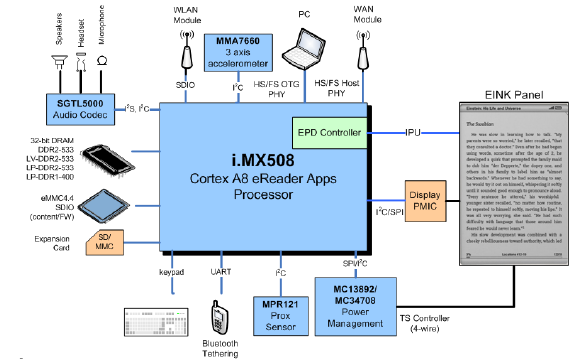
\includegraphics{iMX508.png}
\end{center}


\section{Le contrôleur (EPDC)}

L'EPDC (Electrophoretic Display Controller) conçu spécialement pour les écran E-Ink est une partie importante du processeur iMX508. Il a été intégré directement à l'architecture ARM pour de meilleures performances et une dépense d'énergie moindre. C'est ce contrôleur qui va faire le lien entre l'écran E-Ink et le processeur.
Avant de parler de l'EPDC il est nécessaire de faire un point sur le fonctionnement des écrans électrophorétiques.

\subsection{Les écrans électrophorétiques}

La liseuse à laquelle nous nous intéressons (Sony PRS-T1) possède un écran utilisant la technologie de l'électrophorétique.

L'écran possède des micro-capsules contenant des particules blanches chargées négativement ainsi que des particules noires chargées positivement. Lorsque l'on applique un champ électrique négatif, les particules blanches et noires se sépares (les blanches vont vers une extrémité de la capsule et les noires vers l'autre). Ainsi avec plusieurs millions de capsules et en appliquant des champs électriques, on peut afficher une image en noire et blanc. Une fois que la capsule à reçu un signal électrique, celle-ci garde son état.

Cette technologie à pour principal avantage sa très faible consommation d'énergie puisqu'une fois l'image chargée, elle reste telle qu'elle sans consommation d'énergie et ne nécessite pas d'éclairage particulier (la lumière ambiante suffit).

\begin{center}
	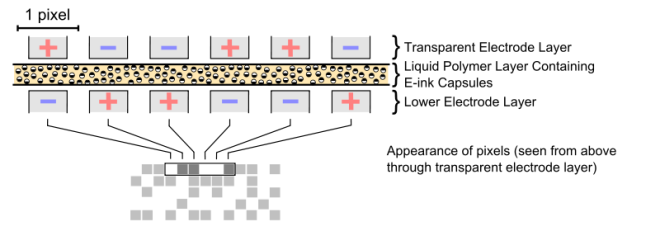
\includegraphics{Electrophoretic.png}
\end{center}


\subsection{Problématique}

Les écrans électrophorétiques nécessite des contrôleurs capables de diriger des ondes (appelées waveforms) pour afficher des images. C'est-à-dire que ces contrôleurs doivent produire un signal (waveform) qui va placer les particules de l'écran de sorte à afficher l'image souhaitée.

Quand une waveform est envoyé, il ne faut pas qu'elle soit perturbée. Concrètement, cela implique qu'il faut bloquer la mémoire du framebuffer utilisé par la waveforme pour ne pas l'altérer.

Il y a trois problèmes majeures pour les écrans électrophorétiques :
\begin{itemize}
	\item[$\bullet$] Comment mapper une mémoire non mappable ?
	\item[$\bullet$] Comment diminuer la latence entre les mises à jour d'affichage ?
	\item[$\bullet$] Comment détecter que l'on a écrit à une adresse mémoire mappée ?
\end{itemize}

Pour résoudre ces problèmes on peut utiliser les Deferred IO.

\subsection{Deferred IO}

Le principe des Deferred IO est le suivant :
\begin{itemize}
	\item Les pages de la mémoire du framebuffer sont initialement marquées en lecture seule.
	\item Quand une application tente d'écrire sur une de ces pages, un défaut de page est créé.
	\item Chaque défauts de page est mis dans une file.
	\item Quand la page mémoire est disponible on écrit ce que l'application voulait dans à la bonne adresse mémoire dans l'ordre des défauts de pages de la file. 
\end{itemize} 

Si on reprends les trois problèmes posés plus haut, le premier (mapper une mémoire non mappable) est résolu puisque lorsque l'on ne peut pas accéder à la mémoire du framebuffer, les écritures vont être mises de côté puis exécutées quand cela sera possible. 
Il n'y a pas de perte de latence puisque écrire dans le framebuffer est aussi rapide que d'écrire dans la mémoire, le second problème est donc résolu.
Le troisième problème est lui aussi résolu puisque l'adresse mémoire qui à généré un défaut de page est connu.
\subsection{Caractéristiques principales de l'EPDC}

\begin{itemize}
	\item[$\bullet$] Résolution jusqu'à 4096 x 4096 pixels à 20 Hz et 2048 x 1536 à 106 Hz
	\item[$\bullet$] De 5 à 32 niveaux de pixels
	\item[$\bullet$] Peux mettre à jour jusqu'à 16 régions sur un écran
	\item[$\bullet$] Mise a jour partielle ou totale de l'écran 
	\item[$\bullet$] Interfaçage avec la mémoire du processeur pour garantir un taux de rafraîchissement
	\item[$\bullet$] Peux réduire sa consommation d'énergie
\end{itemize}


%pré-requis : notion de deferred_io, lookup table (LuT), waveforme
%a supprimer : framebuffer si vu plus tôt
\section{Le driver E-Ink}

\subsection{notions générales}
La liseuse SONY PRS-T1 dispose de quatre éléments hardware et software afin 
de rendre possible l'affichage sur écran E-Ink. Le framebuffer, le pixel pipeline (pxp), l'accès direct à la mémoire (dma) et les lookup tables.

%La notion de framebuffer étant déja expliquer dans la partie  <partie> je ne vais présenter que le pixel pipeline est l'accès mémoire direct
\subsubsection{le framebuffer}

La notion de framebuffer permet l'accès à une zone mémoire contenant l'image affichée actuellement à l'écran sans être dépendante du matériel utilisé en aval.

Le framebuffer utilisé dans le cas d'un écran e-ink se base sur la notion de deferred io vu plus tôt.
%inserer la partie correspondante ? sinon inserer une description du deferred_io

\subsubsection{le pixel pipeline}

La plate-forme Freescale (iMX50) dispose d'un enhanced pixel pipeline (ePXP), ce dernier est utilisé pour : 
	\begin{itemize}
		\item[$\bullet$] gérer la transparence
		\item[$\bullet$] faire des rotations d'images
		\item[$\bullet$] faire des agrandissements / réductions d'images\\
	\end{itemize}

Le ePXP dispose en mémoire d'une image de fond mais aussi de calque(s) afin de pouvoir faire des 
mélanges (via la transparence) de chacune d'entre-elles avant d'envoyer le tout à l'écran.

Il est important de noter que l'ePXP ne gère que des blocs d'une taille donnée (par exemple : 8x8 pixels) pour la résolution des zones de transparence.

\subsubsection{l'accès direct a la mémoire (DMA)}

Le DMA permet au matériel d'avoir accès à la mémoire sans que le transfert ne soit géré par le processeur et donc de rester inactif en attendant la fin de l'opération de lecture / écriture.
Le processeur envoie juste un ordre au contrôleur DMA, ce dernier notifiera la fin du transfert via une opération d'interruption.

Ce mode de transfert de données est utilisé lorsque le processeur ou la mémoire ont une différence dans la capacité de traitement (par exemple : le processeur ne pouvant pas gérer le taux de transfert de la mémoire).
%utilité ?
Sur la plate-forme iMX50 le DMA est géré pour le bus AHB, ce dernier étant synchrone le module de gestion AHB-to-APBH bridge implémente donc un contrôleur DMA afin de pouvoir gérer un mode d'échange asynchrone sur ce bus.

\subsubsection{Les lookup tables (LuT)}

Les lookup tables permettent au contrôleur de gérer plusieurs zone de mise à jour de l'écran en même temps, permettant ainsi de contrer la latence dû à la mise à jour de l'écran via les waveforms.

Les LuT représentent chacune une zone de mise à jour de l'écran, cette zone est défini par : 
	\begin{itemize}
		\item[$\bullet$] une taille
		\item[$\bullet$] la fonction de waveform associée
	\end{itemize}
La gestion des zones de mise à jour étant dynamique les Lut peuvent être de tailles variables. Cependant la fonction de waveform peut influer sur le nombre de LuT disponibles car certains modes remettent l'écran à zéro avant de faire une mise à jour.

Lorsque deux zones gérées par les LuT se chevauchent on dit qu'il y a collision. Lors d'une collision 
la zone qui écrase les zones pré-existantes doit attendre que ces dernières aient fini leurs mises à jour. Ce système est établi car on ne doit pas interrompre l'application d'une waveform à une zone de l'écran (et encore moins appliquer deux waveforms en même temps).
\subsection{Organisation du driver}

Le driver s'organise de la manière suivante : 
	\begin{itemize}
		\item[$\bullet$] fonctions d'initialisation du driver
		\item[$\bullet$] fonctions de bas niveau
	\end{itemize}
	
\subsubsection{Fonctions d'initialisation du driver} % changer le nom ??

	Ces fonctions sont communes a tous drivers Linux.
	\begin{itemize}
		\item[$\bullet$] mxc\_epdc\_fb\_probe : \\
		initialisation du driver mis en place des fonctions de callback, du gestionnaire d'interruption
		\item[$\bullet$] mxc\_epdc\_fb\_exit :\\
		dés-allocation des ressources du noyau pour ce driver
	\end{itemize}
	Le driver dispose aussi de fonctions prenant en charge les événement de gestion d'alimentation (mis en veille, réveil, extinction).
	
\subsubsection{Fonctions de bas niveau}

Les fonctions de bas niveau s'occupent de toutes l'interaction avec le matériel (contrôleur EPD, pixel pipeline, LuT).
Ces fonctions disposent d'accès direct au registre du matériel via les appels à \_\_raw\_writel et \_\_raw\_readl, ce sont les seules fonctions à disposer d'un accès direct au matériel.


%utilité du listing ??
Ces fonctions peuvent être organisées en sous-catégories : 

\begin{itemize}
\renewcommand{\labelitemi}{$\bullet$}
	\item fonctions d'initialisation de paramètre du contrôleur : 
		\begin{itemize}
		\renewcommand{\labelitemi}{$\to$}
			\item epdc\_clock\_gatting
			\item epdc\_set\_screen\_res
			\item epdc\_init\_settings
			\item epdc\_init\_sequence
			\item epdc\_set\_horizontal/vertical\_timing
			\item epdc\_set\_temp
			\item epdc\_set\_border\_gpio
		\end{itemize}
	\item fonctions de gestion des LuT : 
		\begin{itemize}
			\item epdc\_lut\_complete\_intr
			\item epdc\_is\_lut\_complete
			\item epdc\_is\_lut\_active
			\item epdc\_any\_luts\_available
			\item epdc\_get\_next\_lut
			\item epdc\_is\_collision
			\item epdc\_get\_collision\_luts
		\end{itemize}
	\item fonctions de gestion du buffer de travail (au sein du PxP) : 
		\begin{itemize}
			\item epdc\_working\_buf\_intr
			\item epdc\_clear\_working\_buf
			\item epdc\_eof\_intr
			\item epdc\_signal\_eof
			\item epdc\_is\_working\_buffer\_busy
			\item epdc\_is\_working\_buffer\_complete
		\end{itemize}
	\item fonctions de gestion des mises à jour (updates) : 
		\begin{itemize}
			\item epdc\_set\_update\_addr
			\item epdc\_set\_update\_dimension
			\item epdc\_set\_update\_coord
			\item epdc\_submit\_update
		\end{itemize}
	\item le gestionnaire d'interruption et fonctions d'interruptions : 
	\begin{itemize}
		\item epdc\_irq\_handler
		\item epdc\_clear\_eof\_irq
		\item epdc\_clear\_lut\_complete\_irq
	\end{itemize}
\end{itemize}

\subsubsection{Les fonctions de gestion du framebuffer}

Ces fonctions permettent de prendre en charge toute la gestion du framebuffer avec deferred\_io 
propre au contrôleur d'écran E-Ink.
Ce framebuffer gère les particularités des écrans E-Ink : 
	\begin{itemize}
		\item gestion de la température
		\item gestion des waveforms
		\item latence importante de l'écran
	\end{itemize}

Le driver dispose aussi d'une gestion des ioctl pour le framebuffer.
Les ioctl permettent dans les système UNIX d'ajouter des fonctionnalités qui ne seraient pas accessibles autrement (dans notre cas les fonctionnalités propres aux écrans E-Ink).

Le driver implémente les ioctls grâce à la fonction mxc\_epdc\_fb\_ioclt, cette fonction permet l'accès à toutes les fonctionnalités du framebuffer depuis l'espace utilisateur.


\section{Caractéristiques de la liseuse Sony PRS-T1}

\begin{itemize}
		\item[$\bullet$] Processeur : Freescale iMX508
		\item[$\bullet$] Dimensions : 173 x 110 x 8.9 mm
		\item[$\bullet$] Poids : 168 g
		\item[$\bullet$] Ecran :
			\begin{itemize}
				\item Taille : 15,5 cm de diagonal (6")
				\item Résolution : Jusqu'à 16 niveaux de gris
			\end{itemize}
		\item[$\bullet$] Mémoire : 2 Go en interne, extension possible de 32 Go via microSD
		\item[$\bullet$] Batterie : Lithium-ion (tient environ un mois)
		\item[$\bullet$] Interfaces : USB
		\item[$\bullet$] Formats e-book supportés : EPUB, PDF, TXT
		\item[$\bullet$] Formats audio supportés : MP3, AAC
		\item[$\bullet$] Sans-fil : WiFi
		
\end{itemize}

\begin{figure}[h!]
	\begin{center}
		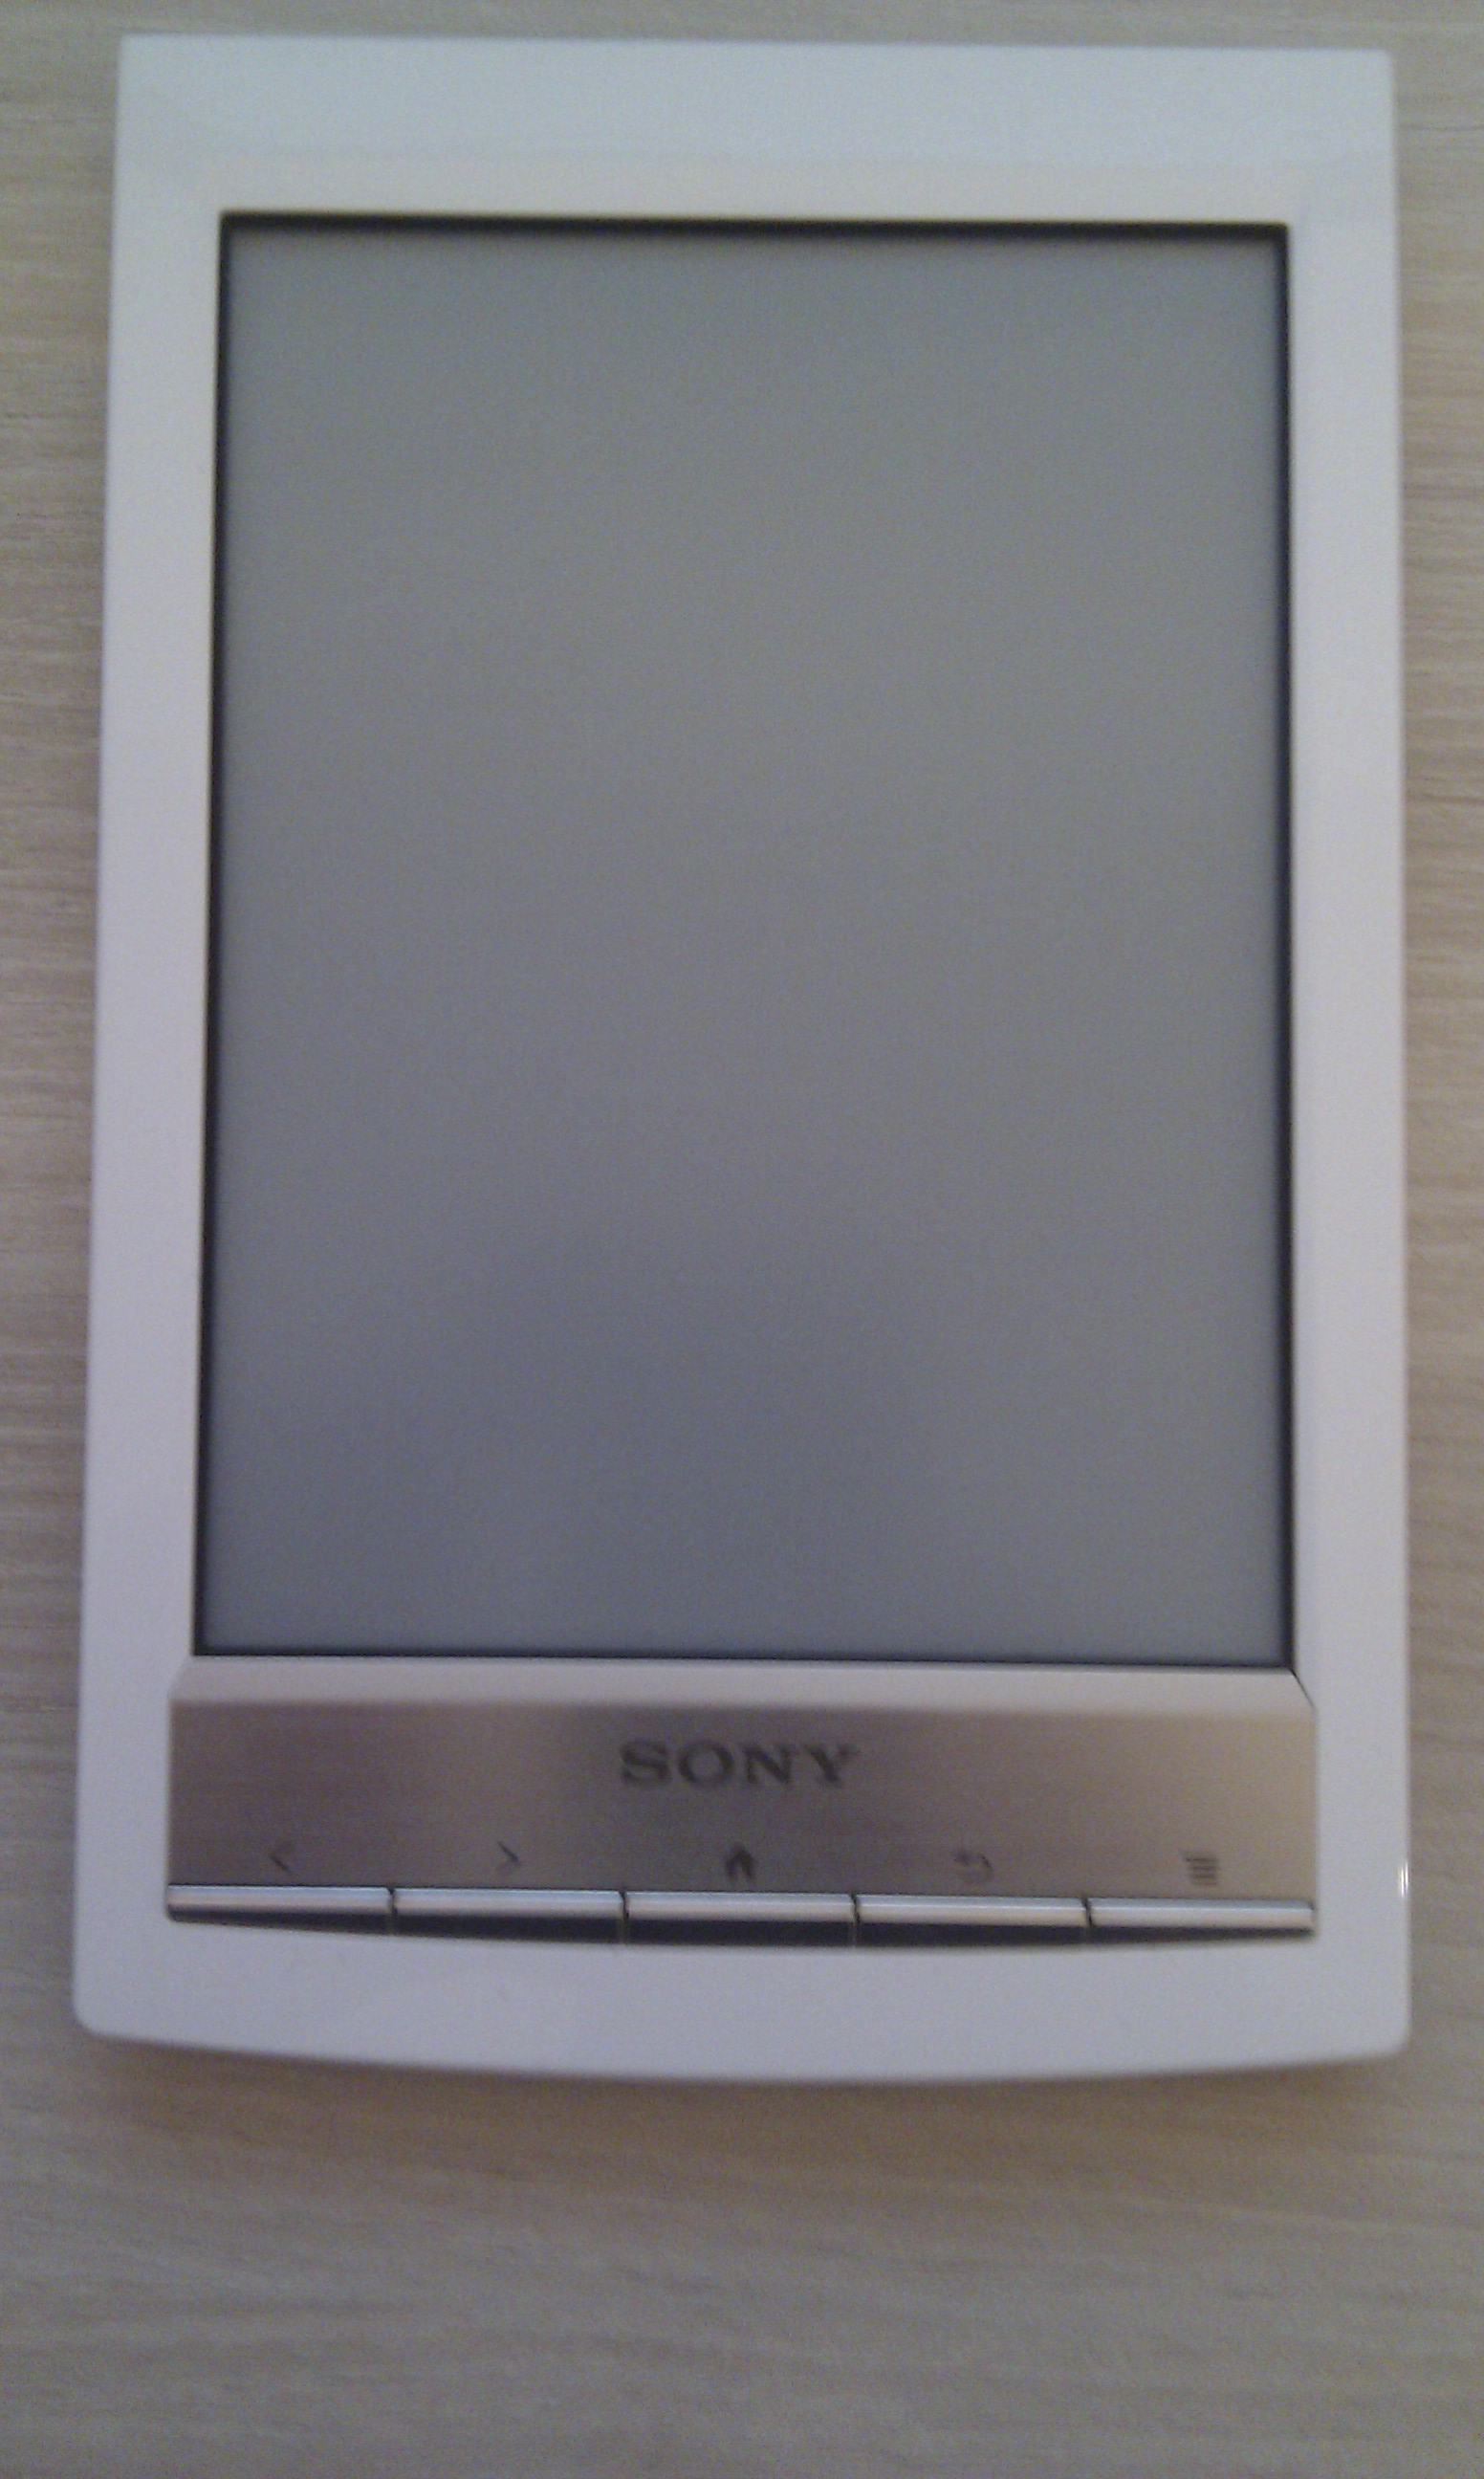
\includegraphics[scale=0.08]{LiseuseSonyPRST1.jpg}
		\caption{Liseuse Sony PRS-T1}
	\end{center}
\end{figure}
